\chapter{Preliminaries}\label{sec:pre}
In this section, the fundamental concepts and definitions necessary 
to contextualize the main contributions of this work are presented. 
I, first, introduce Message Sequence Charts (MSC), followed by 
an examination of communication models that are particularly interesting. 
Then, the notions of Global Type and Realizability are 
defined within the scope of this work, along with the foundational 
elements required to understand the theoretical contributions.

% First, I introduce a formal definition of MSCs, as this will serve as
% a foundation for establishing their connection with Global Types in
% one of the main contributions of this work.
\section{MSCs and Communication Models}

\begin{definition}[Message Sequence Chart]
Let $\mathbb{P}$ be a finite set of processes and $\mathbb{M}$ a set of messages.  
An MSC over $(\mathbb{P}, \mathbb{M})$ is a tuple
$M = (\mathcal{E}, \rightarrow, \vartriangleleft, \lambda)$ where:
$\mathcal{E}$ is a finite (possibly empty) set of \emph{events};
$\lambda : \mathcal{E} \to \Sigma$ is a \emph{labelling function} assigning an action to each event;
$\rightarrow$ and $\vartriangleleft$ are binary relations on $\mathcal{E}$ satisfying the conditions below.
The projection of an MSC $M$ onto a process $i \in \mathbb{P}$ is denoted by $M|_i$.
For each process $p \in \mathbb{P}$, define
$\mathcal{E}_p = \{\, e \in \mathcal{E} \mid \lambda(e) \in \Sigma_p \,\}$
as the set of events executed by $p$.
\begin{enumerate}
    \item \textbf{Process relation.}  
    The relation $\rightarrow \subseteq \mathcal{E} \times \mathcal{E}$ relates an event to its immediate successor on the same process:
    $\rightarrow \;=\; \bigcup_{p \in \mathbb{P}} \rightarrow_p$
    where $\rightarrow_p \subseteq \mathcal{E}_p \times \mathcal{E}_p$ is the direct successor relation of a total order on $\mathcal{E}_p$.

    \item \textbf{Message relation.}  
    The relation $\vartriangleleft \subseteq \mathcal{E} \times \mathcal{E}$ relates matching send/receive events, satisfying:
    \begin{itemize}
        \item For every $(e,f) \in \vartriangleleft$, there exist processes $p,q \in \mathbb{P}$ and a message $m \in \mathbb{M}$ such that  
        $\lambda(e) = \mathrm{send}(p,q,m)$ and $\lambda(f) = \mathrm{rec}(p,q,m)$.
        \item For every receive event $f$ with $\lambda(f) = \mathrm{rec}(p,q,m)$, there exists exactly one $e \in \mathcal{E}$ such that $e \vartriangleleft f$.
        \item For every send event $e$ with $\lambda(e) = \mathrm{send}(p,q,m)$, there exists at most one $f \in \mathcal{E}$ such that $e \vartriangleleft f$.
    \end{itemize}

    \item \textbf{Happens-before relation.}  
    The \emph{happens-before} relation is defined as
    $\le_{\mathrm{hb}} \;=\; (\rightarrow \,\cup\, \vartriangleleft)^{*}$
    and is required to be a partial order on $\mathcal{E}$.
\end{enumerate}
\end{definition}


With MSCs, \cite{di2023partial} presents some interesting communication
semantics. I will describe a few of them informally, using examples to
highlight the differences from the main semantics considered in this work,
which is \verb|synch|, that is also the only one formally defined in 
Definition~\ref{def:synch}. Some examples are
shown in Figure~\ref{fig:msc_examples}. These examples can be verified that 
are really part of the corresponding communication semantics with an online
tool for MSC~\cite{MSCTool}. Figure~\ref{fig:coms} shows a hierarchy
of the communication semantics defined.

\begin{figure}[!ht]
\centering
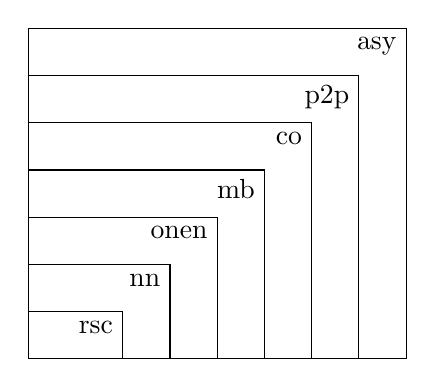
\begin{tikzpicture}[scale=0.6]
  % list of labels in order (from smallest to largest)
%   \def\labels{{rsc,nn,onen,mb,co,p2p,asy}}
  % loop to draw nested squares
  \foreach [count=\i] \lab in {rsc,nn,onen,mb,co,p2p,asy} {
    \draw (0,0) rectangle (\i+1,\i);
    \node[anchor=north east] at (\i+1,\i) {\lab};
  }
\end{tikzpicture}
\caption{Hierarchy of communication model semantics.}
\label{fig:coms}
\end{figure}

First, we introduce the definition of a linearization of an MSC. A
linearization represents a possible ordering of the events in the distributed
system, that is, a way to schedule the events of an MSC.

\begin{definition}[Linearization of a MSC]
	Let $M = (\mathcal{E}, \Rightarrow, \triangleleft, \lambda)$ be an MSC.
	A \emph{linearization} of $M$ is a (reflexive) total order
	$\rightsquigarrow \subseteq \mathcal{E} \times \mathcal{E}$ such that
	$\leq_{hb} \subseteq \rightsquigarrow$.
\end{definition}

\begin{figure}[!ht]
    \centering
    \begin{tabular}{cc}
        \scalebox{0.6}{%
        \begin{msc}[draw frame=none, draw head=none, msc keyword=, 
                    head height=0px, label distance=0.5ex, 
                    foot height=0px, foot distance=0px]{}
            \declinst{p}{p}{}
            \declinst{q}{q}{}

            \mess[pos=0.2]{$m_1$}{p}{q}[2]
            \nextlevel
            \mess[pos=0.8]{$m_2$}{p}{q}
        \end{msc}%
        } &
        \scalebox{0.5}{%
        \begin{msc}[draw frame=none, draw head=none, msc keyword=, 
                    head height=0px, label distance=0.5ex, 
                    foot height=0px, foot distance=0px]{}
            \declinst{p}{p}{}
            \declinst{q}{q}{}
            \declinst{r}{r}{}

            \mess[pos=0.15]{$m_1$}{p}{r}[3]
            \nextlevel
            \mess[pos=0.8]{$m_2$}{p}{q}
            \nextlevel
            \mess[pos=0.8]{$m_3$}{q}{r}
        \end{msc}%
        } \\
        (a) asynchronous (\verb|asy|) & (b) peer-to-peer (\verb|p2p|) \\
        \scalebox{0.5}{%
        \begin{msc}[draw frame=none, draw head=none, msc keyword=, 
                    head height=0px, label distance=0.5ex, 
                    foot height=0px, foot distance=0px]{}
            \declinst{p}{p}{}
            \declinst{q}{q}{}
            \declinst{r}{r}{}
            \declinst{s}{s}{}

            \mess[pos=0.1]{$m_4$}{p}{s}[4]
            \nextlevel
            \mess[pos=0.8]{$m_1$}{p}{q}
            \nextlevel
            \mess[pos=0.2]{$m_2$}{r}{q}
            \nextlevel
            \mess[pos=0.8]{$m_3$}{r}{s}
        \end{msc}%
        } &
        \scalebox{0.6}{%
        \begin{msc}[draw frame=none, draw head=none, msc keyword=, 
                    head height=0px, label distance=0.5ex, 
                    foot height=0px, foot distance=0px]{}
            \declinst{p}{p}{}
            \declinst{q}{q}{}
            \declinst{r}{r}{}

            \mess{$m_1$}{p}{q}
            \nextlevel
            \mess{$m_2$}{q}{r}
        \end{msc}%
        } \\
        (c) mailbox (\verb|mb|) & (d) synchronous (\verb|synch|)
    \end{tabular}
    \caption{MSCs' Examples for various communication models.}
    \label{fig:msc_examples}
\end{figure}

\paragraph{Fully asynchronous}

In the fully asynchronous communication model (\verb|asy|), messages can be 
received at any time after they have been sent, and send events are 
non-blocking. This model can be viewed as an unordered ``bag'' in which 
all messages are stored and retrieved by processes when needed. It is also 
referred to as \emph{non-FIFO}. The formal definition coincides with that of 
an MSC. Figure~\ref{fig:msc_examples}.a illustrates an example of asynchronous 
communication.

\paragraph{Peer-to-peer} 
In the peer-to-peer (\verb|p2p|) communication model, any two messages sent from one 
process to another are always received in the same order as they are sent.
Alternative names are FIFO. An example is shown in Figure~\ref{fig:msc_examples}.b.

% A p2p-MSC is an MSC $M = (E,\to, \lhd, \lambda)$ where, for any two send events $s$ 
% and $s'$ such that $\lambda(s) \in \text{send}(p, q, \_), \lambda(s') in \text{send}(p, q, \_)$, 
% and $s \to^+ s'$, one of the following holds:
% - either $s, s' \in \text{matched}(M)$ with $s \lhd r$ and $s' \lhd r'$ and 
% $r \to^+ r'$,
% - or $s' \in \text{unmatched}(M)$.
% Note that we cannot have two messages $m 1$ and $m 2$, both sent by $p$ to $q$, 
% in that order, such that $m 1$ is unmatched and $m 2$ is matched; unmatched 
% message $m 1$ excludes the reception of any later message.

\paragraph{Causally ordered}
In the causally ordered (\verb|co|) communication model, messages are delivered 
to a process in accordance with the causal dependencies of their emissions. 
In other words, if there are two messages $m_1$ and $m_2$ with the same recipient, 
such that there exists a causal path from $m_1$ to $m_2$, then $m_1$ must be received 
before $m_2$. This notion of causal ordering was first introduced by Lamport under the 
name ``happened-before'' relation. In Figure~\ref{fig:msc_examples}.b, this 
causality is violated: $m_1$ should be received before $m_3$. Causal delivery 
is commonly implemented using Lamport's logical clock algorithm \cite{lamport2019time}.

% An MSC $M = (E, \to, \lhd, \lambda)$ is causally ordered if, for any two send $s$ and 
% $s'$, such that $\lambda(s) \in \text{send}(\_, q, \_), \lambda(s') \in \text{send}(\_, q, \_)$, and 
% $s \leq_{\text{hb}} s'$:
% - either $s, s' \in \text{matched}(M)$ and $r \to^* r'$, with $r$ and $r'$ receive 
% events such that $s \lhd r$ and $s' \lhd r'$.
% - or $s' \in \text{unmatched}(M)$.

% Note that in a \verb|co|-MSC we cannot have two send events $s$ and $s'$ addressed 
% to the same process, such that $s$ is unmatched, $s'$ is matched, and 
% $s \leq_{\text{hb}} s'$.

\paragraph{Mailbox}
In this model, any two messages sent to the same process, regardless of the sender, 
must be received in the same order as they are sent. If a process receives $m_1$ 
before $m_2$, then $m_1$ must have been sent before $m_2$. \verb|mb| coordinates all 
the senders of a single receiver. This model is also called FIFO $n-1$.
In Figure~\ref{fig:msc_examples}.c, an example for this communication model is shown.

% An MSC $M = (E, \to, \lhd, \lambda)$ is a \verb|mb|-MSC if it has a linearization 
% $\rightsquigarrow$ where, for any two send events $s$ and $s'$, such 
% that $\lambda (s) \in \text{send}(\_,q,\_), \lambda (s') \in \text{send}(\_,q,\_)$, and 
% $s \rightsquigarrow s'$
% - either $s,s' \in \text{matched}(M)$ and $r \rightsquigarrow r'$, where 
% $s \lhd r$ and $s' \lhd r'$,
% - or $s' \in \text{unmatched}(M)$.

\paragraph{FIFO 1-n}
This model (\verb|onen|) is the dual of \verb|mb|, it coordinates a sender with all the 
receivers. Any two messages sent by a process must be received in the same 
order as they are sent. These two messages might be received by different 
processes and the two receive events might be concurrent.

% An MSC $M = (E, \to, \lhd, \lambda)$ is a \verb|onen|-MSC if it has a linearization 
% $\rightsquigarrow$ where, for any two send events $s$ and $s'$, such 
% that $\lambda (s) \in \text{send}(p,\_,\_), \lambda (s') \in \text{send}(p,\_,\_)$ and 
% $s \to^+ s'$ (which implies $s \rightsquigarrow s'$)
% - either $s,s' \in \text{matched}(M)$ and $r \rightsquigarrow r'$, with 
% $r$ and $r'$ receive events such that $s \lhd r$ and $s' \lhd r'$,
% - or $s' \in \text{unmatched}(M)$.

\paragraph{FIFO n-n}
In this model (\verb|nn|), messages are globally ordered and delivered according to 
their emission order. Any two messages must be received in the same order 
as they are sent. These two messages might be sent or receives by any process 
and the two send or receive events might be concurrent. The FIFO \verb|n-n| 
coordinates all the senders with all the receivers.

% An MSC $M = (E, \to, \lhd, \lambda)$ is a \verb|nn|-MSC if it has a linearization 
% $\rightsquigarrow$ where, for any two send events $s$ and $s'$, such 
% that $s \rightsquigarrow s'$
% - either $s, s' \in \text{matched}(M)$ and $r \rightsquigarrow r'$, with $r$ 
% and $r'$ receive events such that $s \lhd r$ and $s' \lhd r'$,
% - or $s' \in \text{unmatched}(M)$.

\paragraph{Synchronous}
The synchronous (\verb|synch|) communication model imposes 
the existence of a scheduling such that any send event is 
immediately followed by its corresponding receive event. 
An example for this communication model is shown in Figure~\ref{fig:msc_examples}.d.

% An MSC $M = (E, \to, \lhd, \lambda)$ is an \verb|rsc|-MSC if it has no unmatched 
% send events and there is a linearization $\rightsquigarrow$ where any 
% matched send event is immediately followed by its respective receive event.
	
\begin{definition}[$\acommunicationmodel$-linearisable MSC]\label{def:linearisable-msc}
	An MSC $\mmsc$ is \textit{linearisable} in a communication model $\acommunicationmodel$
	if $\linearisationsof{\mmsc}{\acommunicationmodel}\neq\emptyset$.
	We write $\mscsetofmodel{\acommunicationmodel}$ for the set of all MSCs 
	linearisable in $\acommunicationmodel$.
\end{definition}

Finally, let's formally define what is a \verb|synch|-MSCs in this context.

\begin{definition}[Synchronous execution]\label{def:synch}
	An execution $\execution=(w,\source) \in \executionsofmodel{\synchmodel}$
	if for all send event $s\in\sendeventsof{e}$, $s+1$ is a receive event
	of $e$ and $\source(s+1)=s$.
\end{definition}

In other words, an MSC $M$ belongs to $\mscsetofmodel{\synchmodel}$ if
all send events are immediately followed by their corresponding receive events.

\section{Basic notions for Global Types}
This part will further highlight the basic notion to understand the formal proof 
for the theorem presented in Section~\ref{sec:proof} and, in particular, Global Type
and Weakly-realizable. We begin by extending the definition of linearisability so 
that it applies to all communication models.
In our setting, Global Types are automata that describe a language of MSCs.

\begin{definition}[Global Type]
	An \emph{arrow} is a triple $(p,q,m)\in\Procs\times\Procs\times\Messages$ 
	with $p\ne q$; we often write $\marrow{p}{q}{m}$ instead of $(p,q,m)$, and 
	write $\labelalphabet$ to denote the finite set of arrows.
	A Global Type $\gt$ is a deterministic finite state automaton over the 
	alphabet $\labelalphabet$.
\end{definition}

\begin{example}
An example of a Global Type expressed as an automaton is the following.
Consider the not-implementable specification stated in 
Listing~\ref{lst:not-impl-exm}. The protocol can be modelled with the 
Global Type in Figure~\ref{fig:gt-exm}.

\begin{figure}[!ht]
	\centering
	\begin{tikzpicture}[node distance=1.5cm, auto, scale=0.7]
		\node[state, initial, initial text={}] (s0) {1};
			\node[state] (s1) [above right=of s0] {2};
			\node[state] (s2) [below right=of s0] {3};
			\node[state,accepting] (s3) [right=of s1] {4};
			\node[state,accepting] (s4) [right=of s2] {5};

			\draw[->] (s0) to node[above,sloped]{$\gtlabel{A}{B}{x}$}(s1);
			\draw[->] (s0) to node[above,sloped]{$\gtlabel{A}{B}{y}$}(s2);
			\draw[->] (s1) to node[above,sloped]{$\gtlabel{C}{D}{z}$}(s3);
			\draw[->] (s2) to node[above,sloped]{$\gtlabel{C}{D}{w}$}(s4);
			
		\end{tikzpicture}
		\caption{A Global Type, which respects the specification given in Listing~\ref{lst:not-impl-exm}.}
		\label{fig:gt-exm}
	\end{figure}
\end{example}

%% TODO: scrivere per bene definizione di automi A e cosa vuol dire il prod

% \begin{definition}[Product $L(\prod_i A_i)$]
% We associate with $A=\prod_i A_i$ the language of possible executions of
% the automaton $A$, denoted $L(A)$. For any set of concurrent automata $A_i$,
% the language $L(\prod_i A_i)$ of the product of the automata contains
% only complete and well-formed words. Furthermore, for a given MSC $M$,
% the language $L(\prod_i A_i)$ either contains all linearization of
% $M$ or it contains none.
% \end{definition}

% ------------------------existential MSC language------------------------

% A Global Type defines a language of MSCs in two different ways, one
% existential and one universal. Let $\labellanguageof{\gt}$ be the set of
% sequences of arrows $w$ accepted by $\gt$. Note that for $w \in \Arrows^*$,
% the function $w \mapsto \labeltomsc{w}$ with
% $\labeltomsc{w} \in \mscsetofmodel{\synchmodel}$ is not injective, as two
% arrows with disjoint pairs of processes commute. We write $w_1 \sim w_2$ if
% $\labeltomsc{w_1} = \labeltomsc{w_2}$, and $[w]$ for the equivalence class
% of $w$ with respect to $\sim$.

I can now formally define the relationship between MSCs and Global Types. 
Intuitively, Global Types represent a set of MSCs, allowing us to reason 
about multiple message sequence scenarios. To obtain this result, let's 
define what is the existential MSC language $\existentialmsclanguageof{\gt}{}$ 
of a Global Type. Let $\labellanguageof{\gt}$ be the set of
sequences of arrows $w$ accepted by $\gt$.
Informally, the existential MSC language $\existentialmsclanguageof{\gt}{}$ of a 
Global Type $\gt$ is the set of MSCs that admit at least one representation as a
sequence of arrows in $\labellanguageof{\gt}$.
% , and the universal MSC
% language $\universalmsclanguageof{\gt}$ of a Global Type $\gt$ is the set of
% MSCs whose representations as sequences of arrows are all in
% $\labellanguageof{\gt}$:
\begin{definition}[$\existentialmsclanguageof{\gt}$]
	$$
		\existentialmsclanguageof{\gt} \eqdef \{\labeltomsc{w} \mid
		w \in \labellanguageof{\gt}\} %% \qquad
		% \universalmsclanguageof{\gt} \eqdef \{\labeltomsc{w} \mid
		% [w] \subseteq \labellanguageof{\gt}\}.
	$$
\end{definition}

There is also the universal MSC language $\universalmsclanguageof{\gt}$ 
of a Global Type $\gt$, defined as the set of MSCs whose arrow-sequence 
representations all belong to $\labellanguageof{\gt}$. However, a formal 
definition is not necessary here. 

% \begin{definition}[Commutation-closed]
%     A Global Type $\gt$ is \emph{commutation-closed} if
%     $$
%     \existentialmsclanguageof{\gt} = \universalmsclanguageof{\gt}.
%     $$
% \end{definition}
% We write $\msclanguageofcc{\gt}$ for the common language.

I now introduce the definition of implementability following the one given 
by Alur, et al. \cite{alur2005realizability}, referred to as 
\textit{Weak-realizability}.
To formalize it, we first define the notions of 
\textit{weak implication} and \textit{weak closure}.

%% TODO: Spiegare meglio con intuizioni

\begin{definition}[Weakly-imply]
	Let $\setmsc$ be a set of MSCs and $M$ another MSC. $\setmsc$
	\textit{weakly implies} $M$, if for any sequence of automata
	$\langle A_i \ |\ 1\leq i\leq n\rangle$, if every MSC in $\setmsc$ is in
	$L(\prod_i A_i)$ then so is $M$ in $L(\prod_i A_i)$.
\end{definition}

In order to understand the meaning of \emph{weak implication},
consider the following example.

\begin{example}
Define two MSCs, MSC1 and MSC2. Both perform the same four
communications, but in different orders.  
MSC1 first sends message $a$ from P1 to P2, then from P1 to P3, 
then sends $b$ from P4 to P2, and finally from P4 to P3.  
MSC2 instead starts with P4 sending $b$ to P2, then to P3, 
followed by P1 sending $a$ to P2 and then to P3.  

Now define a third MSC $M$ with the same four messages but in a
different order: P1 sends $a$ to P2, P4 sends $b$ to P2, P4 sends 
$b$ to P3, and finally P1 sends $a$ to P3.  

We say $M$ is weakly implied by MSC1 and MSC2. Indeed, by looking
at each process projection we recover the same behavior in one of
them: for P1 and P4 in both, for P2 in MSC1, and for P3 in MSC2.  
Figure~\ref{fig:weak-impl} illustrates the three MSCs.

\begin{figure}[!ht]
\centering
\begin{tabular}{ccc}
\begin{minipage}{0.32\textwidth}
\scalebox{0.55}{%
\begin{msc}[left environment distance=0cm, draw frame=none, draw head=none, msc keyword=, head height=0px, label distance=0.5ex, foot height=0px, foot distance=0px]{}
	\declinst{P1}{P1}{}
	\declinst{P2}{P2}{}
	\declinst{P3}{P3}{}
	\declinst{P4}{P4}{}

	\mess{a}{P1}{P2}
	\nextlevel
	\mess[pos=0.25]{a}{P1}{P3}
	\nextlevel
	\nextlevel
	\mess[pos=0.25]{b}{P4}{P2}
	\nextlevel
	\mess{b}{P4}{P3}
\end{msc}
} 
\end{minipage}
&
\begin{minipage}{0.32\textwidth}
\scalebox{0.55}{%
\begin{msc}[left environment distance=0cm, draw frame=none, draw head=none, msc keyword=, head height=0px, label distance=0.5ex, foot height=0px, foot distance=0px]{}
	\declinst{P1}{P1}{}
	\declinst{P2}{P2}{}
	\declinst{P3}{P3}{}
	\declinst{P4}{P4}{}

	\mess[pos=0.25]{b}{P4}{P2}
	\nextlevel
	\mess{b}{P4}{P3}
	\nextlevel
	\nextlevel
	\mess{a}{P1}{P2}
	\nextlevel
	\mess[pos=0.25]{a}{P1}{P3}
\end{msc}
}
\end{minipage}
&
\begin{minipage}{0.32\textwidth}
\scalebox{0.55}{%
\begin{msc}[left environment distance=0cm, draw frame=none, draw head=none, msc keyword=, head height=0px, label distance=0.5ex, foot height=0px, foot distance=0px]{}
	\declinst{P1}{P1}{}
	\declinst{P2}{P2}{}
	\declinst{P3}{P3}{}
	\declinst{P4}{P4}{}

	\mess{a}{P1}{P2}
	\nextlevel
	\mess[pos=0.25]{b}{P4}{P2}
	\nextlevel
	\nextlevel
	\mess{b}{P4}{P3}
	\nextlevel
	\mess[pos=0.25]{a}{P1}{P3}
\end{msc}
}
\end{minipage} \\
MSC1 & MSC2 & $M$
\end{tabular}
\caption{The MSC $M$ is weakly implied by MSC1 and MSC2}
\label{fig:weak-impl}
\end{figure}
\end{example}

\begin{definition}[Weakly-closure $\setmsc^w$]
	The weak-closure $\setmsc^w$ of a set $\setmsc$ of MSCs contains all the MSCs
	$\setmsc$ weakly implies.
\end{definition}

\begin{definition}[Weakly-realizable]
	An MSC $M$ is said to be weakly-realizable if the set of MSCs
	$L(M)$ is weakly realizable. A set of MSCs $\setmsc$ is said to be weakly
	realizable if $\setmsc=\setmsc^w$.
\end{definition}
It is important to note that this definition does not include the
property of deadlock-freedom. 

% CINZIA, X TESI:
% sarebbe interessante mettere la definizione di PPDP e mostrare 
% l'equivalenza tra le due

% VERSIONE ALTERNATIVA
% \begin{definition}[Projection]
% For an MSC $M$ and a process $P_i$, let $M|_i$ denote the sequence of events be
% belonging to the process $P_i$ in $M$.
% \end{definition}
% \begin{definition}[Weakly-imply]
% The set of MSCs $\setmsc$ weakly implies an MSC $M$ iff for all $1\leq i\leq n$, there
% exist an MSC $M_i\in L$ such that $M|_i=M_i|_i$
% \end{definition}
% \begin{definition}[Weakly-realizable]
% ? TODO ?
% \end{definition}

We are now ready to present the main contributions of this work.


